
\documentclass[11pt]{article}
\usepackage[margin=1in]{geometry}
\usepackage{graphicx}
\usepackage{amsmath,amssymb}
\usepackage{booktabs}
\usepackage{float}
\usepackage{hyperref}
\usepackage[numbers,sort&compress]{natbib}
\usepackage{caption}
\usepackage{setspace}
\hypersetup{colorlinks=true,linkcolor=black,citecolor=black,urlcolor=blue}
\setstretch{1.12}
\title{Claim-Bounded Diagnostics for Noise-Assisted Annealing and Frustration Boundaries in a Reduced Active-Particle Feedback Surrogate\\\large v0.3.0 Synthesis Addendum}
\author{Keiji Yoshimura\\\small Independent Researcher}
\date{May 25, 2026}
\begin{document}
\maketitle
\begin{center}
\small
Repository: \href{https://github.com/yokken0907/active-particle-feedback-kinetic-arrest}{github.com/yokken0907/active-particle-feedback-kinetic-arrest}\\
Historical repository DOI context: \href{https://doi.org/10.5281/zenodo.20202120}{10.5281/zenodo.20202120}\\
License: source-defined Evaluation-Only Notice in the repository.
\end{center}

\begin{abstract}
This addendum summarizes a claim-bounded v0.2.0--v0.2.6 audit sequence for a reduced active-particle feedback surrogate originally framed around kinetic-arrest-like behavior and noise-induced annealing. The locked synthesis is conservative: within the implemented toy-model setting, a noise-assisted annealing window was observed across multiple tested conditions, and local feedback was sometimes competitive or beneficial relative to null controls. However, the effect was not uniquely attributable to local feedback, and high-frustration geometries produced first-class failure boundaries. By v0.2.6, formerly persistent boundaries split into rescue-stable and persistent-hard-boundary regimes under targeted relief, with extreme frustration remaining unrecovered in the tested setting. This addendum does not claim experimental active-matter validation, biological or social-system validation, crowd-control or civilization-engineering interpretation, a universal kinetic-arrest mechanism, or local feedback as a uniquely necessary annealing generator.
\end{abstract}

\paragraph{Reader guidance and claim boundary.}
The intended reading is as a reduced active-particle surrogate diagnostic. The work is adjacent to active matter and self-propelled particle modeling \cite{vicsek1995,marchetti2013,bechinger2016,cates2015,fily2012,redner2013}, but the present addendum is not an experimental active-matter paper. It also does not validate social, biological, crowd-control, or civilization-scale interpretations. The allowed claims are limited to noise-window diagnostics, feedback-geometry dependence, frustration-boundary classification, and rescue-stability behavior inside the tested toy-model setting.

\section{Synthesis of the audit sequence}
The v0.2.0--v0.2.6 sequence was designed as a claim-boundary audit rather than as a positive-only validation campaign. Early stages tested whether a noise-assisted annealing window could be seen in a reduced surrogate and whether local feedback was necessary for that window. Later stages froze the window, tested holdout geometries, introduced frustration boundaries, attempted targeted rescue, and finally classified persistent boundaries.

The terminal synthesis lock found all seven expected phases and fixed the decision as \texttt{PASS-APFKA-V030-SYNTHESIS-LOCKED}. The terminal v0.2.6 audit recorded four native failure boundaries, seven rescue-stable classifications, no conditional-rescue cases, and one persistent hard boundary. The mean native local-minus-no-feedback score was 0.1254227, while the mean best-minus-native gain on native failures was 1.2053399. These results support a bounded diagnostic claim: local feedback can be competitive or useful in some geometries, but the robustly reported object is a noise-window and frustration-boundary diagnostic, not a universal feedback-induced arrest theory.

\section{Boundary and rescue classification}
\begin{table}[H]
\centering
\caption{Terminal v0.2.6 boundary classification used in the v0.3.0 synthesis. Scores are dimensionless surrogate diagnostics.}
\begin{tabular}{lrrl}
\toprule
Topology & Native score & Best score & Classification\\
\midrule
extreme\_frustration\_holdout & -1.5878 & -0.8117 & persistent hard boundary\\
frustrated\_checker\_phase\_shift & -1.1662 & 0.2224 & rescue stable\\
frustrated\_checker\_v2 & -0.8548 & 0.5698 & rescue stable\\
striped\_domains\_holdout\_v2 & -0.2875 & 0.9446 & rescue stable\\
mixed\_basin\_holdout\_v2 & 0.8781 & 1.1916 & rescue stable\\
modular\_patchy\_holdout & 1.0555 & 1.3201 & rescue stable\\
random\_sparse\_holdout & 0.8849 & 1.1438 & rescue stable\\
smooth\_gradient\_holdout & 0.5135 & 0.8354 & rescue stable\\
\bottomrule
\end{tabular}
\end{table}

The most important negative result is the persistent hard boundary in the extreme-frustration holdout. Targeted relief improved the score from -1.5878 to -0.8117, but the best policy still failed the pass condition. This prevents overstatement: the surrogate contains an interpretable failure boundary rather than a universal repair mechanism.

\begin{figure}[H]
\centering
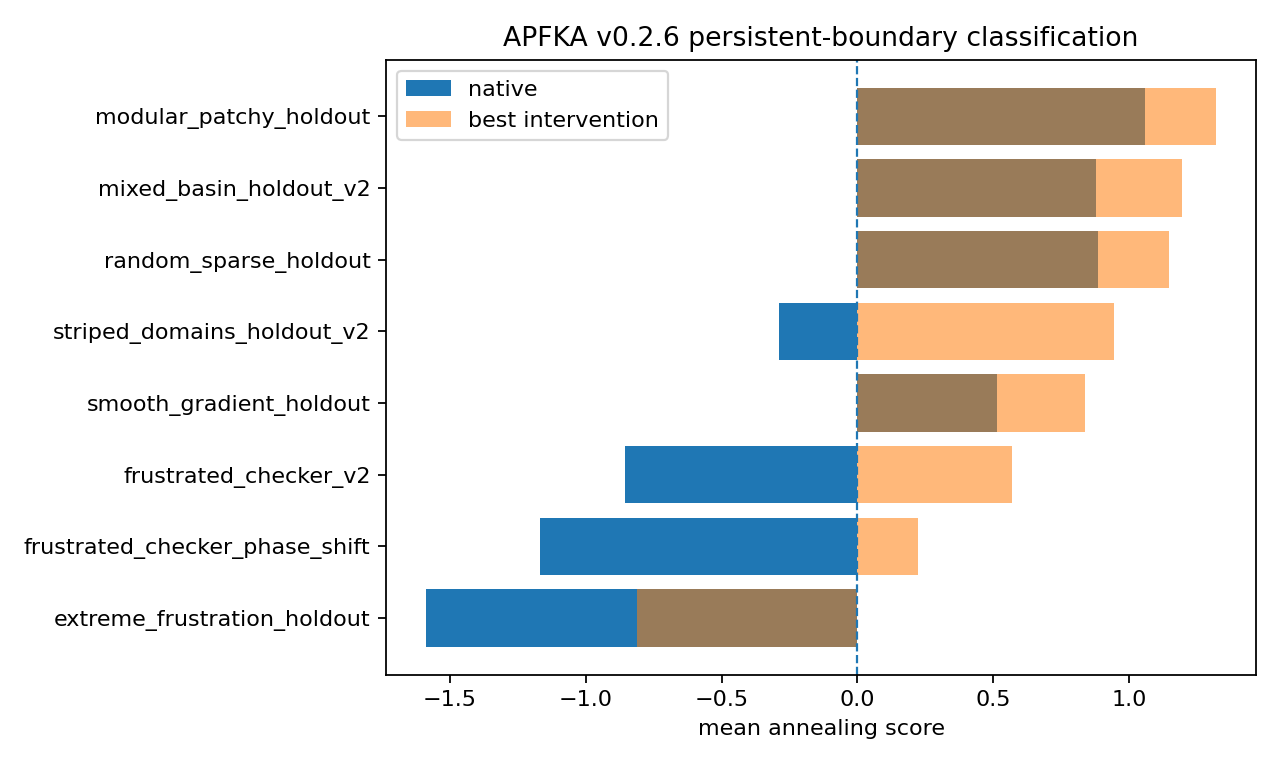
\includegraphics[width=0.86\linewidth]{v0_2_6_apfka_v026_boundary_scores.png}
\caption{Terminal boundary-score comparison from v0.2.6. The figure is included as evidence for rescue-stable and persistent-hard-boundary separation, not as an experimental active-matter result.}
\end{figure}

\begin{figure}[H]
\centering
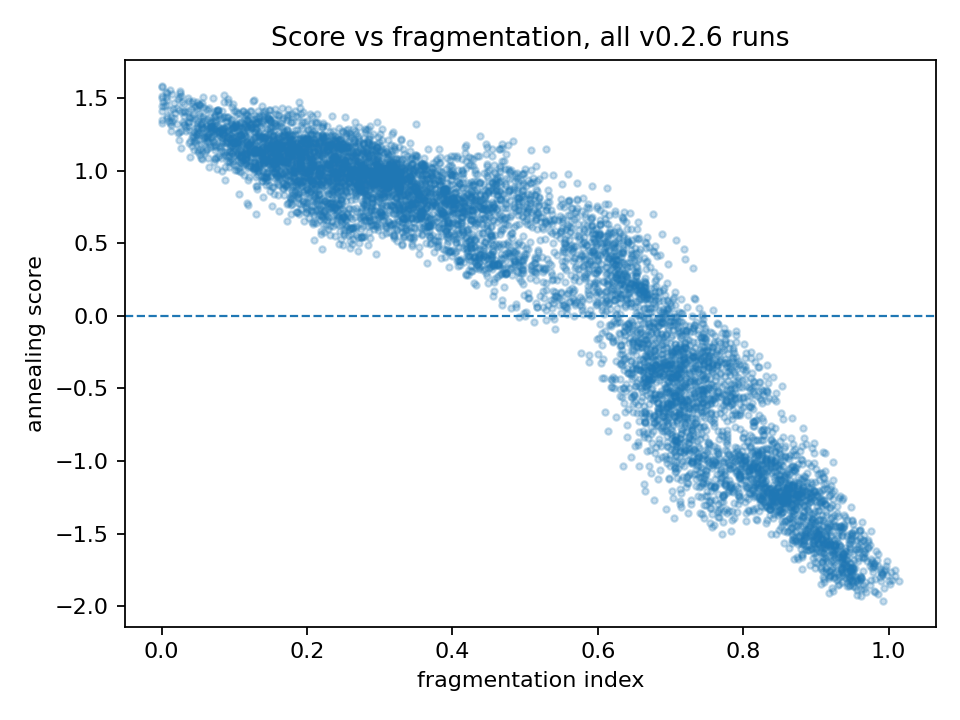
\includegraphics[width=0.86\linewidth]{v0_2_6_apfka_v026_score_vs_fragmentation.png}
\caption{Score-fragmentation diagnostic from the terminal boundary classification. The pattern supports a surrogate-level classification of frustration and rescue stability within the tested implementation.}
\end{figure}

\section{Interpretation}
The locked interpretation is deliberately narrower than the original broad metaphor of social or civilization-scale defragmentation. The present addendum does not use the surrogate to make social-system claims. Instead, the result is a model-internal diagnostic: a noise-assisted annealing window appears across tested conditions, local feedback is geometry-dependent, and high-frustration geometries can split into rescue-stable and persistent-hard-boundary regimes.

This framing is scientifically useful because it preserves both positive and negative evidence. It reports where the surrogate produces annealing-window behavior, where feedback is beneficial but not uniquely causal, and where even targeted rescue remains insufficient.

\section{Limitations}
The following interpretations are explicitly excluded. This addendum does not claim experimental validation in active matter, biological validation, social-system validation, crowd-control or swarm-control deployment, civilization-engineering guidance, policy applicability, a universal kinetic-arrest theorem, or a proof that local feedback is necessary for noise-induced annealing. The figures and tables are diagnostic artifacts of the implemented reduced surrogate.

\section*{AI assistance disclosure}
The author used AI assistance for drafting, code generation, numerical-audit scaffolding, and manuscript preparation. The author remains responsible for the final claim boundary, interpretation, and release decisions.

\begin{thebibliography}{9}
\bibitem{vicsek1995} T. Vicsek, A. Czirok, E. Ben-Jacob, I. Cohen, and O. Shochet, ``Novel Type of Phase Transition in a System of Self-Driven Particles,'' \emph{Physical Review Letters}, 75, 1226--1229, 1995. DOI: \href{https://doi.org/10.1103/PhysRevLett.75.1226}{10.1103/PhysRevLett.75.1226}.
\bibitem{marchetti2013} M. C. Marchetti et al., ``Hydrodynamics of soft active matter,'' \emph{Reviews of Modern Physics}, 85, 1143--1189, 2013. DOI: \href{https://doi.org/10.1103/RevModPhys.85.1143}{10.1103/RevModPhys.85.1143}.
\bibitem{bechinger2016} C. Bechinger et al., ``Active particles in complex and crowded environments,'' \emph{Reviews of Modern Physics}, 88, 045006, 2016. DOI: \href{https://doi.org/10.1103/RevModPhys.88.045006}{10.1103/RevModPhys.88.045006}.
\bibitem{cates2015} M. E. Cates and J. Tailleur, ``Motility-Induced Phase Separation,'' \emph{Annual Review of Condensed Matter Physics}, 6, 219--244, 2015. DOI: \href{https://doi.org/10.1146/annurev-conmatphys-031214-014710}{10.1146/annurev-conmatphys-031214-014710}.
\bibitem{fily2012} Y. Fily and M. C. Marchetti, ``Athermal Phase Separation of Self-Propelled Particles with No Alignment,'' \emph{Physical Review Letters}, 108, 235702, 2012. DOI: \href{https://doi.org/10.1103/PhysRevLett.108.235702}{10.1103/PhysRevLett.108.235702}.
\bibitem{redner2013} G. S. Redner, M. F. Hagan, and A. Baskaran, ``Structure and Dynamics of a Phase-Separating Active Colloidal Fluid,'' \emph{Physical Review Letters}, 110, 055701, 2013. DOI: \href{https://doi.org/10.1103/PhysRevLett.110.055701}{10.1103/PhysRevLett.110.055701}.
\end{thebibliography}
\end{document}
